\documentclass[10pt,table]{beamer}
\usepackage[utf8]{luainputenc}
\usepackage[ngerman]{babel}


%\usetheme[block=fill]{m}                     % Use metropolis theme
\usepackage{beamerthemeuzl-conference}

\usepackage{Alegreya,AlegreyaSans}

\logo{
\includegraphics[scale=.62]{uzl-logo-ITCS.pdf}}
\usepackage{amsmath}
\DeclareMathOperator*{\argmin}{arg\,min}
\usepackage{nicefrac}
\usepackage{algorithm}
\usepackage{dsfont}
\usepackage{subfig}
\usepackage{mathtools}
\usepackage{graphicx}
\usepackage{mathpazo} 
\usepackage{tikz}

% Finn
\usepackage{xspace}
\usepackage{float}
\usepackage{subfig}
\usepackage{color, colortbl}
\definecolor{uzlred}{HTML}{BF0000}
\definecolor{uzlgreen}{HTML}{008000}
\definecolor{uzlpurple}{HTML}{700080}
\newcommand{\highlightrow}{\rowcolor{Ozeangruen!5}}

% mine
\usepackage{mathtools}
\usepackage{algpseudocode}
\usetikzlibrary{positioning, shapes, snakes, automata}
\usepackage{transparent}
\setbeamercovered{transparent}

\title{Algorithmen für das Moving-Target Travelling Salesman Problem}
%\subtitle{}
\author{Felix Greuling}
\date{27.01.2019}


\begin{document}
\maketitle


%\iffalse
\begin{frame}{Überblick}
\tableofcontents[hideallsubsections]
\end{frame}

\AtBeginSection[]
{
  \begin{frame}
    \frametitle{Überblick}
    \tableofcontents[currentsection, hideallsubsections]
  \end{frame}
}
%\fi

\AtBeginSection[]{
  \begin{frame}[noframenumbering]
  \vfill
  \centering
  \begin{beamercolorbox}[sep=8pt,center,shadow=true,rounded=true]{title}
    \usebeamerfont{title}\insertsectionhead\par%
  \end{beamercolorbox}
  \vfill
  \end{frame}
}



\section{Einleitung}
\begin{frame}{Einleitung}
Travelling Salesman Problem (TSP)
\begin{itemize}
\item
Optimierungsproblem aus der Kombinatorik
\item
Reihenfolge an Zielen, sodass die Tourzeit minimal ist
\item
Tour startet und endet im selben Ziel
\item
NP-vollständig
\end{itemize}
\end{frame}

\begin{frame}{Einleitung}
\begin{center}
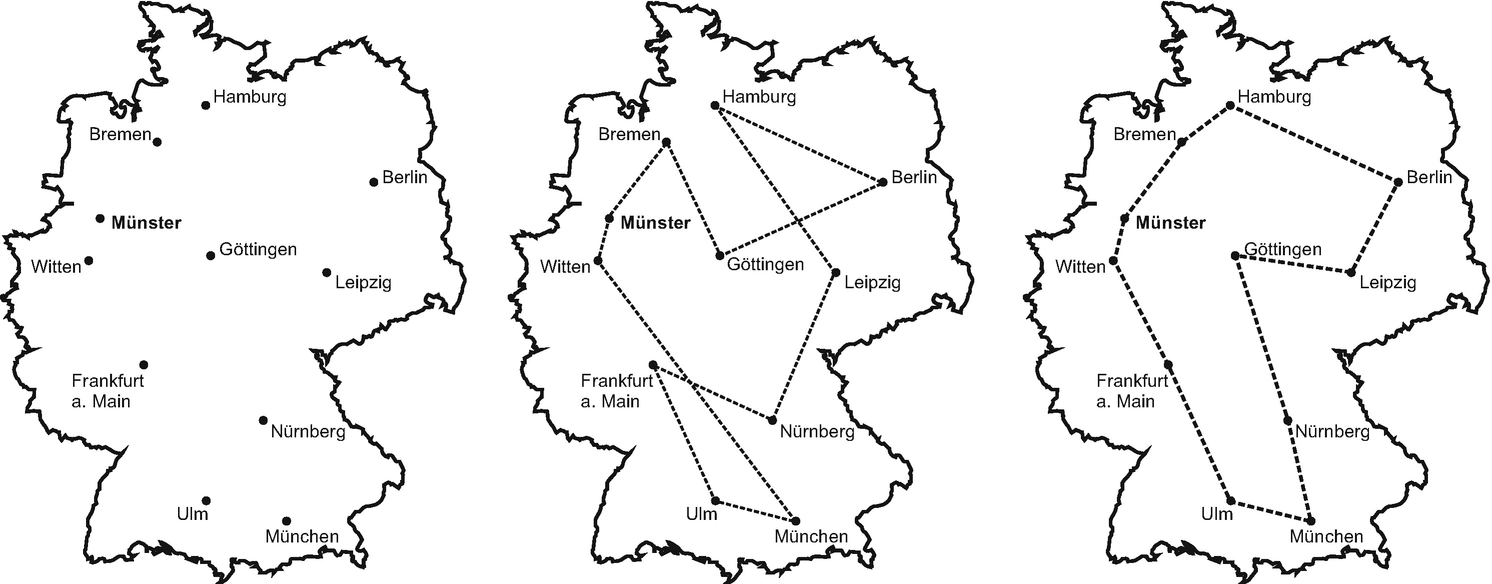
\includegraphics[scale=0.8]{Images/TSP.png}\\~\\
\end{center}
\end{frame}

\begin{frame}{Einleitung}
Moving-Target-TSP (MT-TSP)
\begin{itemize}
\item
Im Jahre 1998 von Helvig et al. erwähnt.
\item
Ziele sind nun nicht mehr stationär
\item
Problematik bleibt die selbe
\end{itemize}

\end{frame}

\begin{frame}{Einleitung}
\centering
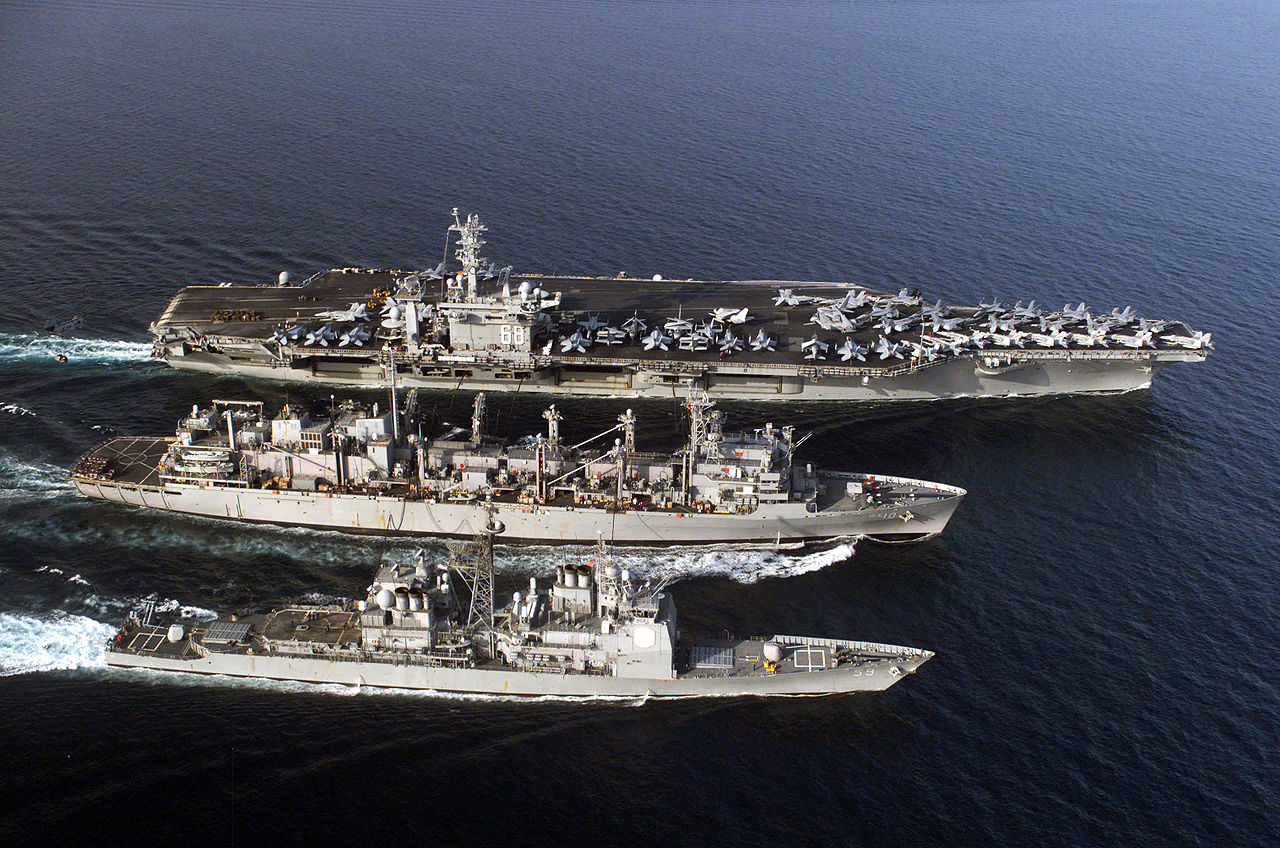
\includegraphics[scale=0.8]{Images/Versorgungsschiff.jpg}
\end{frame}

\section{Grundlagen}
\begin{frame}{MT-TSP}
Formal haben Helvig et al. das Problem wie folgt definiert:\\~\\
\begin{quote}
The moving-target traveling salesman problem: Given a set $S = \{s_1, \dots , s_n\}$ of \emph{targets}, each $s_i$ moving at constant velocity $\overrightarrow{v_i}$ from an initial position $p_i$, and given a \emph{pursuer} starting at the origin and having maximum speed $v>|\overrightarrow{v_i}|$, find the fastest tour starting (and ending) at the origin, which intercepts all targets.
\end{quote}
\end{frame}

\begin{frame}{MT-TSP}
\begin{itemize}
\item Ziele
\begin{align*}
Z = (z_1, ..., z_n)
\end{align*}
\item Startpositionen 
\begin{align*}
P = (p_1, ..., p_n)
\end{align*}
\item Geschwindigkeiten
\begin{align*}
V = (v_1, ..., v_n)
\end{align*}
\item Verfolger
\begin{align*}
\kappa = (p_\kappa,v_\kappa)~~~~
\end{align*}
\end{itemize}
\end{frame}

\begin{frame}{MT-TSP in einer Dimension}
\centering
\scalebox{0.8}{
\begin{tikzpicture}
\coordinate (a) at (-5,0) node[below=0.1cm of a]{-1000};
\coordinate (b) at (-1,0) node[below=0.1cm of b]{-1};
\coordinate (c) at (0,0) node[below=0.1cm of c]{0};
\coordinate (d) at (1,0) node[below=0.1cm of d]{1};
\coordinate (e) at (5,0) node[below=0.1cm of e]{1000};
\coordinate (f) at (-6,0) node[below=0.1cm of f, xshift=3.0cm]{[...]};
\coordinate (g) at (6,0) node[below=0.1cm of g, xshift=-3.0cm]{[...]};
% Geschwindigkeiten
\node[above of=a, xshift=-0.1cm, yshift=0.1cm] {$-1$};
\node[above of=b, xshift=-0.3cm, yshift=0.1cm] {$-8$};
\node[above of=d, xshift=0.3cm, yshift=0.1cm] {$8$};
\node[above of=e, xshift=0.1cm, yshift=0.1cm] {$1$};
\fill (a) circle (2.5pt);
\fill (b) circle (2.5pt);
\fill (d) circle (2.5pt);
\fill (e) circle (2.5pt);
\draw (f)--(a)--(b)--(c)--(d)--(e)--(g);
% links 1.
\coordinate (aa) at (-5,0.8);
\draw (a) -- (aa);
\draw (-5,0.8) -- (-5.2,0.8);
\draw (-5.2,0.9) -- (-5.4,0.8) -- (-5.2,0.7) -- cycle;
% links 2.
\coordinate (bb) at (-1,0.8);
\draw (b) -- (bb);
\draw (-1,0.8) -- (-1.7,0.8);
\draw (-1.7,0.9) -- (-1.9,0.8) -- (-1.7,0.7) -- cycle;
% mitte
\draw (0,2) -- (0,1.5) -- (0.4,1.75) -- cycle;
\coordinate (cc) at (0,2);
\draw (c) -- (cc);
% rechts 2.
\coordinate (dd) at (1,0.8);
\draw (d) -- (dd);
\draw (1,0.8) -- (1.7,0.8);
\draw (1.7,0.9) -- (1.9,0.8) -- (1.7,0.7) -- cycle;
% rechts 1.
\coordinate (ee) at (5,0.8);
\draw (e) -- (ee);
\draw (5,0.8) -- (5.2,0.8);
\draw (5.2,0.9) -- (5.4,0.8) -- (5.2,0.7) -- cycle;
\end{tikzpicture}} \\~\\ 
\begin{itemize}
\item<2,3> Ziele $Z=\{(-1000,-1),(-1,8),(1,8),(1000,1)\}$
\item<2,3> Verfolger $\kappa=(0,10)$ 
\item<3> $Left=\{(-1,8),(-1000,-1)\}$ 
\item<3> $Right=\{(1,8),(1000,1)\}$
\end{itemize}

\end{frame}

\begin{frame}{MT-TSP in einer Dimension}
\begin{itemize}
\item $Left=\{(-1,8),(-1000,-1)\}$ 
\item $Right=\{(1,8),(1000,1)\}$
\item $A=(s_k,s_f)$
\end{itemize}
\pause
\centering
\scalebox{0.8}{\parbox{.5\linewidth}{
\begin{align*}
A_0&=\emptyset\\
A_1&=\{(-1, -8), (1, 8)\} &\text{Index-Summenwert}=0\\
A_2&=\{(1, 8), (-1, -8)\} &\text{Index-Summenwert}=0\\ 
A_3&=\{(-1, -8), (1000, 1)\} &\text{Index-Summenwert}=1~\\
A_4&=\{(1000, 1), (-1, -8)\} &\text{Index-Summenwert}=1~\\
A_5&=\{(-1000, -1), (1, 8)\} &\text{Index-Summenwert}=1~\\
A_6&=\{(1, 8), (-1000, -1)\} &\text{Index-Summenwert}=1~\\
A_7&=\{(-1000, -1), (1000, 1)\} &\text{Index-Summenwert}=2~\\
A_8&=\{(1000, 1), (-1000, -1)\} &\text{Index-Summenwert}=2~\\
A_{9}&=\emptyset
\end{align*}
}}
\end{frame}

\begin{frame}{MT-TSP in einer Dimension}
\begin{figure}
\centering
\scalebox{0.75}{
\begin{tikzpicture}[->]
\node[state] (A0) {$A_0$};
\node[state, above right = of A0, yshift=+1.1cm, xshift=0.2cm] (A1) {$A_1$};
\node[state, below right = of A0, yshift=-1.1cm, xshift=0.2cm] (A2) {$A_2$};
\node[state, above right = of A1, yshift=-0.3cm, xshift=0.6cm] (A5) {$A_5$};
\node[state, below right = of A1, yshift=+0.3cm, xshift=0.6cm] (A6) {$A_6$};
\node[state, above right = of A2, yshift=-0.3cm, xshift=0.6cm] (A3) {$A_3$};
\node[state, below right = of A2, yshift=+0.3cm, xshift=0.6cm] (A4) {$A_4$};
\node[state, right = of A6, xshift=0.6cm] (A7) {$A_7$};
\node[state, right = of A3, xshift=0.6cm] (A8) {$A_8$};
\node[state, right = of A0, xshift = 8cm] (A9) {$A_9$};
\pause
\path (A0) edge [bend left] (A1) node[xshift=0.8cm, yshift=1.5cm] {$\tau_{left}$};
\path (A0) edge [bend right] (A2) node[xshift=0.8cm, yshift=-1.5cm] {$\tau_{right}$};

\path (A1) edge [bend left] (A5) node[xshift=1.1cm, yshift=0.9cm] {$\tau_{left}$};
\path (A1) edge [bend right] (A6) node[xshift=1.1cm, yshift=-0.9cm] {$\tau_{right}$};
\path (A2) edge [bend left] (A3) node[xshift=1.1cm, yshift=0.8cm] {$\tau_{right}$};
\path (A2) edge [bend right] (A4) node[xshift=1.1cm, yshift=-0.9cm] {$\tau_{left}$};

\path (A5) edge [bend left] (A9) node[xshift=3.8cm, yshift=-0.9cm] {$\tau_{final}$};
\path (A4) edge [bend right] (A9) node[xshift=3.8cm, yshift=0.8cm] {$\tau_{final}$};

\path (A6) edge (A7) node[xshift=1.3cm, yshift=+0.2cm] {$\tau_{left}$};
\path (A6) edge (A8) node[xshift=1.0cm, yshift=-0.5cm] {$\tau_{right}$};
\path (A3) edge (A7) node[xshift=1.0cm, yshift=+0.5cm] {$\tau_{left}$};
\path (A3) edge (A8) node[xshift=1.3cm, yshift=-0.2cm] {$\tau_{right}$};

\path (A7) edge (A9) node[xshift=1.1cm, yshift=-0.8cm] {$\tau_{final}$};
\path (A8) edge (A9) node[xshift=1.1cm, yshift=+0.8cm] {$\tau_{final}$};
\end{tikzpicture}}
\end{figure}
\end{frame}

\section{Zwei-orthogonale-Achsen im MT-TSP}
\begin{frame}{Zwei-orthogonale-Achsen im MT-TSP}
\begin{itemize}
\item
Neue Modifikation mit zusätzlicher Achse
\item
Ziele und Verfolger können sich ausschließlich auf dieser bewegen
\item
Dem Verfolger ist es möglich, die Achse zu wechseln

\end{itemize}
\end{frame}

\subsection{Theoretische Grundlagen}
\begin{frame}{Theoretische Grundlagen}
\begin{block}{Lemma 1}
In jeder optimalen Tour bei zwei orthogonalen Achsen im MT-TSP muss sich der Verfolger mit seiner  maximalen Geschwindigkeit bewegen.
\end{block}
\begin{block}{Lemma 2}
In jeder optimalen Tour bei zwei orthogonalen Achsen im MT-TSP gelten für den Verfolger folgende Eigenschaften:
\begin{itemize}
\item
Bewegt sich der Verfolger wegführend vom Ursprung, ändert dieser erst seine Richtung, sofern er das schnellste Ziel in seiner Richtung abgefangen hat.
\item
Bewegt sich der Verfolger in Richtung des Ursprungs, ändert dieser solange nicht seine Richtung, bis er den Ursprung erreicht hat.
\end{itemize}
\end{block}
\end{frame}


\subsection{Heuristiken}
\begin{frame}{Problem der Modellierung als Graphen}

\end{frame}

\begin{frame}{Prioritätsansatz}

\end{frame}

\begin{frame}{Brute-Force-Ansatz}

\end{frame}

\section{Ergebnisse}
\begin{frame}{Ergebnisse}

\end{frame}

\section{Zusammenfassung und Ausblick}
\begin{frame}{Zusammenfassung}
    
\end{frame}

\begin{frame}{Ausblick}

\end{frame}




\nocite{*}
\appendix
\begin{frame}[noframenumbering, plain]
\Large\center
Danke für Ihre Aufmerksamkeit!
\end{frame}


\begin{frame}[allowframebreaks, noframenumbering]{References} 
	\bibliographystyle{amsalpha}
	\bibliography{lit}
\end{frame}

\end{document}
